  {\color{teal!90}\chapter{Bonjour}\label{cap:Bonjour}}

  \AddToShipoutPictureBG*{%
    \AtPageUpperLeft{%
      \raisebox{-\height}{%
        
\includegraphics[width=\paperwidth]{./chapters/bonjour.jpg}%
      }%
    }
  }

  \minitoc % Creating an actual mini table of contents

  \section{Bonjour and Device Discovery}
  \label{sec:Bonjour}

  The purpose of this chapter is to explore the integration of the Bonjour service in Android, specifically focusing on how an Android device must present itself to be recognized as a target by an iOS device, like an iPhone, for services such as AirPlay. Bonjour, Apple's implementation of zero-configuration networking, facilitates automatic service discovery, enabling devices within the same network to discover and connect with each other without manual configuration.

  \begin{wrapfigure}{L}{4cm}
    \centering
    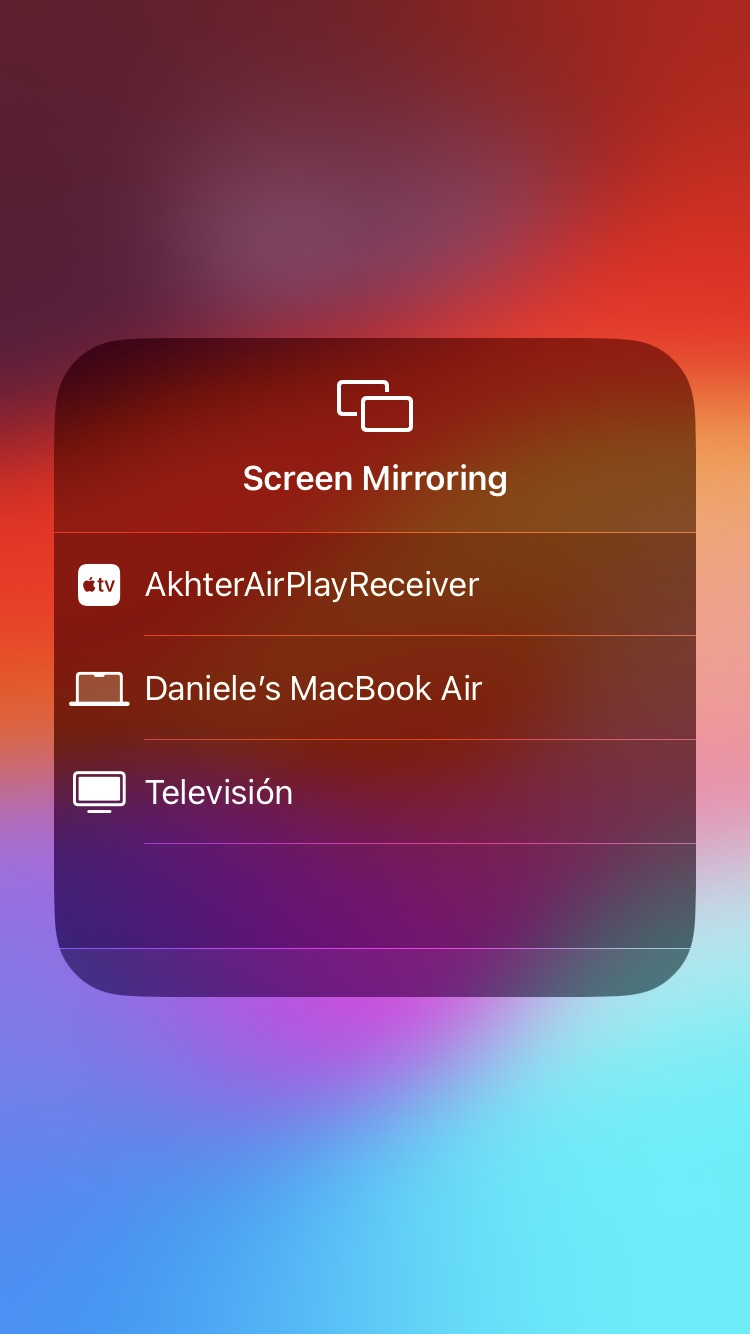
\includegraphics[width=4cm]{./chapters/iPhoneDetecting.jpeg}
    \caption{Representation of iPhone detecting Android device with Bonjour service.}\label{fig:iPhone-detecting}
  \end{wrapfigure}

  Our approach begins with the correct setup of Bonjour on the Android device, defining a JSON response containing essential parameters that describe the device and its capabilities. Initial investigation has highlighted several key parameters that must be included for successful device identification and connection initiation by an iOS device.
  The JSON response, typically returned when the iPhone queries the Bonjour service, needs to specify fields such as \texttt{deviceid}, \texttt{features}, \texttt{flags}, \texttt{model}, and \texttt{srcvers}. These parameters convey the device's unique identity, the capabilities it supports (e.g., AirPlay mirroring), and the protocol versions in use. By accurately configuring these fields, we aim to ensure the Android device can mimic the characteristics of a compatible AirPlay receiver, which are generally expected by iOS.
  Currently, our setup includes a simulated JSON configuration that imitates an AppleTV device, utilizing \texttt{model} values like \texttt{"AppleTV3,2"} and feature flags that signify support for AirPlay mirroring. This configuration has enabled preliminary recognition by the iPhone, but further tests are ongoing to validate full compatibility and to understand the response from the iOS device upon attempting to initiate a mirroring session.